\begin{opin}{\guscolor}{Gustavo}

\subsubsection{Divulgación de las Matemáticas como docentes}

En la clase de hoy Raquel hizo referencia a un debate que puede generar polémica. El asunto es si las matemáticas son asequibles para todo el mundo o solo para elegidos como algunos piensan. Raquel es partidaria de que todo el mundo podría aprender matemáticas correctamente si estas se explican cómo deberían. En mi opinión, yo no afirmaría ni una cosa ni la otra al 100\%, es decir, no todo es blanco ni negro. Relacionándolo con las inteligencias múltiples que explicó Helena López Casares en la conferencia que dio el 20 de septiembre en el Campus Vicálvaro, me atrevería a decir que un profesor puede intentar despertar el interés de un alumno por las matemáticas, pero es cierto que dentro de todas las posibles inteligencias que pueden existir, si un alumno no tiene bien desarrollada la inteligencia relacionada con las matemáticas, un profesor podrá ser capaz de despertasr el interés de un alumno hasta un límite.

En cualquier caso, ya sea para difundir las matemáticas a todo el mundo o no, lo que está claro es que hay que intentar quitar ese estigma existente dentro del mundo matemático acerca de que la gente a la que le gustan las matemáticas son “bichos raros”. Para ello hay que difundir y divulgar las matemáticas y qué mejor manera que hacerlo de un tiempo a esta parte que a través de la prensa y de los medios de comunicación. 

El problema está en que los periodistas históricamente han huido de las matemáticas desde bien entrada la Universidad y por tanto existen muchos errores en prensa y televisión acerca de las matemáticas como se pueden ver en las transparencias de clase o en el video visto en clase de Marilo Montero (\url{https://www.youtube.com/watch?v=zclITKd4ivQ}). Este error tiene que ver con el error o fallo que puede existir a la hora de representar ciertas expresiones matemáticas como puede ser la expresión 48/2(9+3) y que ha generado un debate en los foros de la asignatura que muestro a continuación dado que  me pareció muy interesante y no tuvimos tiempo para abordarlo en clase

En mi opinión, inicialmente el resultado era 2, clarísimamente. Pero después de razonar con mis compañeros de clase vi que podría haber más soluciones aparte de la mia. David Soria explicó lo siguiente: 

\begin{center}\rule{200pt}{0.2pt}\end{center}

El problema tiene dos opciones distintas dependiendo del orden de operación. Hay dos elementos de distinto orden que son PEMDAS Y BEDMAS, según en la escuela que te hayan enseñado puede ser uno u otro. El orden para aplicar las operaciones en PEMDAS (Paréntesis, Eponenciación, Multiplicación, División, Adición y Sustracción) mientras que el orden en BEDMAS (Paréntesis,, Exponenciación, División, Multiplicación, Adición y Sustracción). 

Con PEMDAS el resultado de la operación sería item 

\[
48÷2·(9+3) \to 48 ÷ 2·(12) \to 48÷2·12 \to 48÷24 = 2
\]

Con BEMDAS  el resultado de la operación seria item 

\[
48÷2·(9+3) \to 48 ÷ 2·(12) \to 24·12 = 288
\]

\begin{center}\rule{200pt}{0.2pt}\end{center}


Antonio Jesus Guerrero y Carlos Rodiño entendían que “que multiplicar y dividir están al mismo nivel, igual que sumar y restar; y que en tal caso la prioridad de operación es de izquierda a derecha.”

Posteriormente, Manuel Pulido compartió su forma de pensar con Carlos y con Antonio,  y además corroboró la información con un libro de texto indicando que es la manera más extendida de hacerlo.

El libro de texto decía lo siguiente:

\textit{En general:}

\begin{itemize}
\item \textit{En operaciones con paréntesis, primero hay que realizar las que están entre paréntesis y luego las demás.}
\item \textit{En operaciones sin paréntesis, primero se efectúan las multiplicaciones y divisiones y luego, las sumas y las restas.}
\item \textit{En operaciones de igual prioridad, primero la de más a la izquierda.}
\end{itemize}

\textit{Por lo tanto ellos lo calcularían así:}

\[
48÷2·(9+3) \to 48 ÷ 2·(12) \to 24·12 = 288
\]



Por último, intenté llegar a una conclusión que es la importancia que tiene como colocar las expresiones matemáticas para no dar lugar a ambigüedades de este estilo.


Lo que queda claro es que unos entienden la expresión como $\frac{48}{2(9+3)}$ y otros como $\frac{48}{2}(9+3)$.

Si ambas expresiones se reflejaran así no daría lugar a ninguna confusión.

En cualquier caso no estoy de acuerdo en aplicar las reglas que indican ciertos libros de texto dado que si aplicamos estas reglas indicadas por el libro de texto al que hacía referencia Manual, la expresión 

Podría interpretarse como si fuera igual a 288, cuando todos tenemos claro que debe ser igual a item 

Para terminar el debate Miriam Expóstio indicó que 
\textit{Desde mi punto de vista, para que se entendiese que hay que dividir todo entre "2(9+3)" se tendría que poner todo ese término entre corchetes, no?}


Con lo que estoy totalmente de acuerdo. Y por tanto, al no haber corchetes, el problema lo tiene quien escribe la expresión al haber varias interpretaciones.
Las matemáticas deben ser exactas y no dar lugar a interpretaciones. Para interpretaciones ya están las leyes ;-)
Además de los errores cometidos por los periodistas de manera involuntaria como puede ser el de Mariló también están los errores cometidos intencionadamente con el objetivo de manipular a esa parte de la sociedad menos documentada. Ejemplos pueden ser el número de asistentes a una manifestación que varía en función de diversos intereses.
También hablamos acerca de los errores comunes que tienen los alumnos a la hora de realizar ciertas operaciones básicas en matemáticas y que independientemente de ser de letras o de ciencia, no se deberían cometer. Es como si los de ciencia dijeran que no saben escribir gramaticalmente bien porque son de ciencia. No tiene sentido. La cultura es independiente de ser de ciencias o de letras.
Otra de las formas de divulgar las matemáticas en televisión es a través de series. Por ejemplo:

\begin{itemize}
\item “Universo matemático” era una serie, producida en el año 2000, que constaba de 10 capítulos y que abordaba distintos temas relacionados con la matemática. La obra obtuvo en el año 2002 el Premio a la divulgación científica del Festival Internacional Científico de Pekín. 
\item Se puede ver en 
\href{http://www.rtve.es/alacarta/videos/universo-matematico/} {http://www.rtve.es/alacarta/videos/universo-matematico/} 
\item “Más por menos”. Esta serie consta de 13 programas emitidos de septiembre de 1996 a enero de 1997 y de noviembre de 2002 a enero de 2003 en el programa de Televisión Educativa de TVE-2 "La Aventura del Saber".
\item Se puede ver en 
\href{http://www.rtve.es/television/la-aventura-del-saber/documentales/mas-por-menos/} {http://www.rtve.es/television/la-aventura-del-saber/documentales/mas-por-menos/} 
\item “Orbita Laika” sección de Matemáticas por Raúl Ibañez.
\item Matemáticas invisibles:
\begin{itemize}
\item Curiosidad sobre el tamaño de las hojas DINA-n (
\href{http://www.sabercurioso.es/2008/11/05/por-que-una-hoja-de-papel-din-a4-tiene-el-tamano-que-tiene/}{http://www.sabercurioso.es/2008/11/05/por-que-una-hoja-de-papel-din-a4-tiene-el-tamano-que-tiene/}
)
\item Explicación del digito de control de un código de barras. Todo tiene su explicación
\end{itemize}
\end{itemize}



Como vemos, hay muchas formas de divulgar las matemáticas y nosotros como futuros docentes debemos ser parte fundamental en el futuro de esta divulgación, ya sean:

\begin{itemize}
\item Artículos en revistas  
\item Convocatorias de actividades relacionadas con las matemáticas (fotografía, concursos, juegos…)
\item Concesiones de premios (Medalla Fields) 
\item Iniciativas como dar publicidad a los congresos internacionales de matemáticas 
\item Promover jornadas de popularización y divulgación  (“olimpiadas matemáticas”) 
\item Museos (Museo Nacional de Ciencia y tecnología, MUNCYT, antiguo Cosmocaixa)) 
\item Páginas web divulgativas
\item Divulgamat (
\href{http://www.divulgamat.net/}{http://www.divulgamat.net/}
)
\end{itemize}

\begin{minipage}[hbtp]{1.0\linewidth}
	\centering
	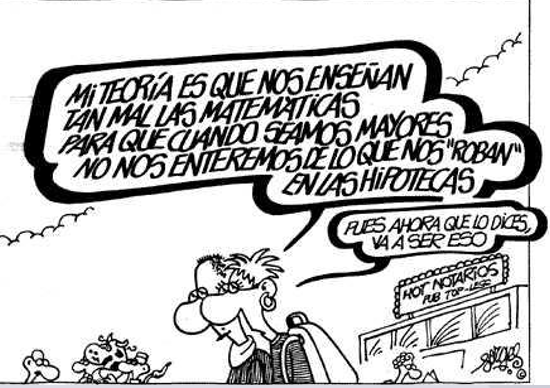
\includegraphics[width=0.6\linewidth]{img/chistegus.png}
	%\captionof{figure}{Coche de mediadios del siglo pasado.}
\end{minipage}

\end{opin}






\begin{opin}{\victorcolor}{Víctor}

En mi diario incluía también una mención sobre el ejemplo $48÷2·(9+3)$ tratado por mi compañero Gustavo, pero lo voy a omitir por evitar repeticiones innecesarias.

\subsubsection{Docentes como divulgadores}

Me ha resultado muy novedosa la idea de que \textit{los profesores deberíamos ser los primeros divulgadores de las Matemáticas} (Antonio Durán). 
%
No sólo en el aula con los alumnos, sino también fuera de ella.
%
Hacen falta personas apasionadas por las Matemáticas, capaces de ayudar a la gente a romper el mito ``Es que soy de letras'' 
%
\footnote{Al igual que personas apasionadas por las letras que rompan con el mito ``Es que soy de ciencias''. Qué pasa, ¿que por ser de ciencias no saber redactar ni expresarte por escrito?}
%
Y a veces, ese argumento se utiliza para escaquearse de llevar las cuentas en un viaje o en una cena, cuyos cálculos no pasan de simples divisiones y sumas que un estudiante de 5º de Primaria podría hacer.

\subsubsection{Construyendo el conocimiento matemático sin lagunas}

En verano estuve de voluntariado en Perú y una semana fue dar clase de mates a chavales de secundaria de allí. 
%
Les ocurría que sabían despejar las ecuaciones perfectamente. Hacían todos los pasos bien, hasta que al llegar al final, $3x = 24 \to x=\frac{24}{3} = ?$. 
%
El último paso no eran capaces de hacerlo. ¿Cómo es posible que lleguen al curso en el que están y sepan despejar sin saberse las tablas de multiplicar? 
%
¡Qué sistema educativo tan ineficiente! 
%
Pasan de curso sin los conocimientos necesarios... construyen el conocimiento con unas lagunas bestiales.

Viendo los errores de primero de grado propuestos por Raquel me doy cuenta que no hay tanta diferencia entre el modelo de allí, con el modelo de aquí; 
%
en cuanto a construir un conocimiento sólido sin lagunas.


La Ted Talk de Salman Khan me parece una charla que todo docente de Matemáticas debería ver (tanto es así, que mi primera aportación a los foros de la asignatura fue plantear esta charla).
%
¿Te imaginas construir el tejado de un edificio sin haber terminado los cimientos?
%
Nadie trabaja así. Ni siquiera nadie, exceptuando a Fito y Fitipaldis, sugiere trabajar así.
%
¿Porqué en Matemáticas enseñamos a integrar sin que se haya interiorizado bien la derivada? ¿Porqué tratamos de enseñar diagonalizar matrices sin que los alumnos tengan claro cómo se factoriza un polinomio con Ruffini?
%
No digo que haya que enseñar Ruffini en la universidad, sino que los docentes en la secundaria nos esforcemos por no dejar lagunas en el conocimiento de los alumnos. 
%
``Enseñar para la maestría'', como dice Salman Khan.

\paragraph{Khan Academy}

Al hilo de retomar esta charla este curso (ya la conocía anteriormente) estuve paseando por la web y viendo los recursos que tienen.
%
Es una pena que esté en inglés y tal vez no sea utilizable en clase, pero ayuda a hacerse una idea de cómo funcionar. 
%
Además, están trabajando en traducciones, para hacer llegar la academia a más países.

Otro aprendizaje, al hilo de Khan, es la importancia del inglés. 
%
Más allá de poder comunicarse, en internet hay infinidad de recursos (empezando por las charlas Ted) que merecen mucho la pena y que se podrían estar aprovechando mucho más, si supiéramos inglés.
%
A raíz de esto, cuando me preguntan qué es lo que más valoro del inglés, lo que siempre contesto es: ``poder aprender autodidactamente de lo que sea en internet y acceder a reflexiones y conocimiento de otras personas''.


\end{opin}

\begin{opin}{\pedrocolor}{Pedro}

\subsubsection{La clase invertida - jornada complementaria}
\vspace{2.0cm}
\end{leftbar}
\vspace{-2.0cm}
\begin{figure}[hbtp]
\begin{leftbar}{\pedrocolor}
\vspace{1cm}
\centering
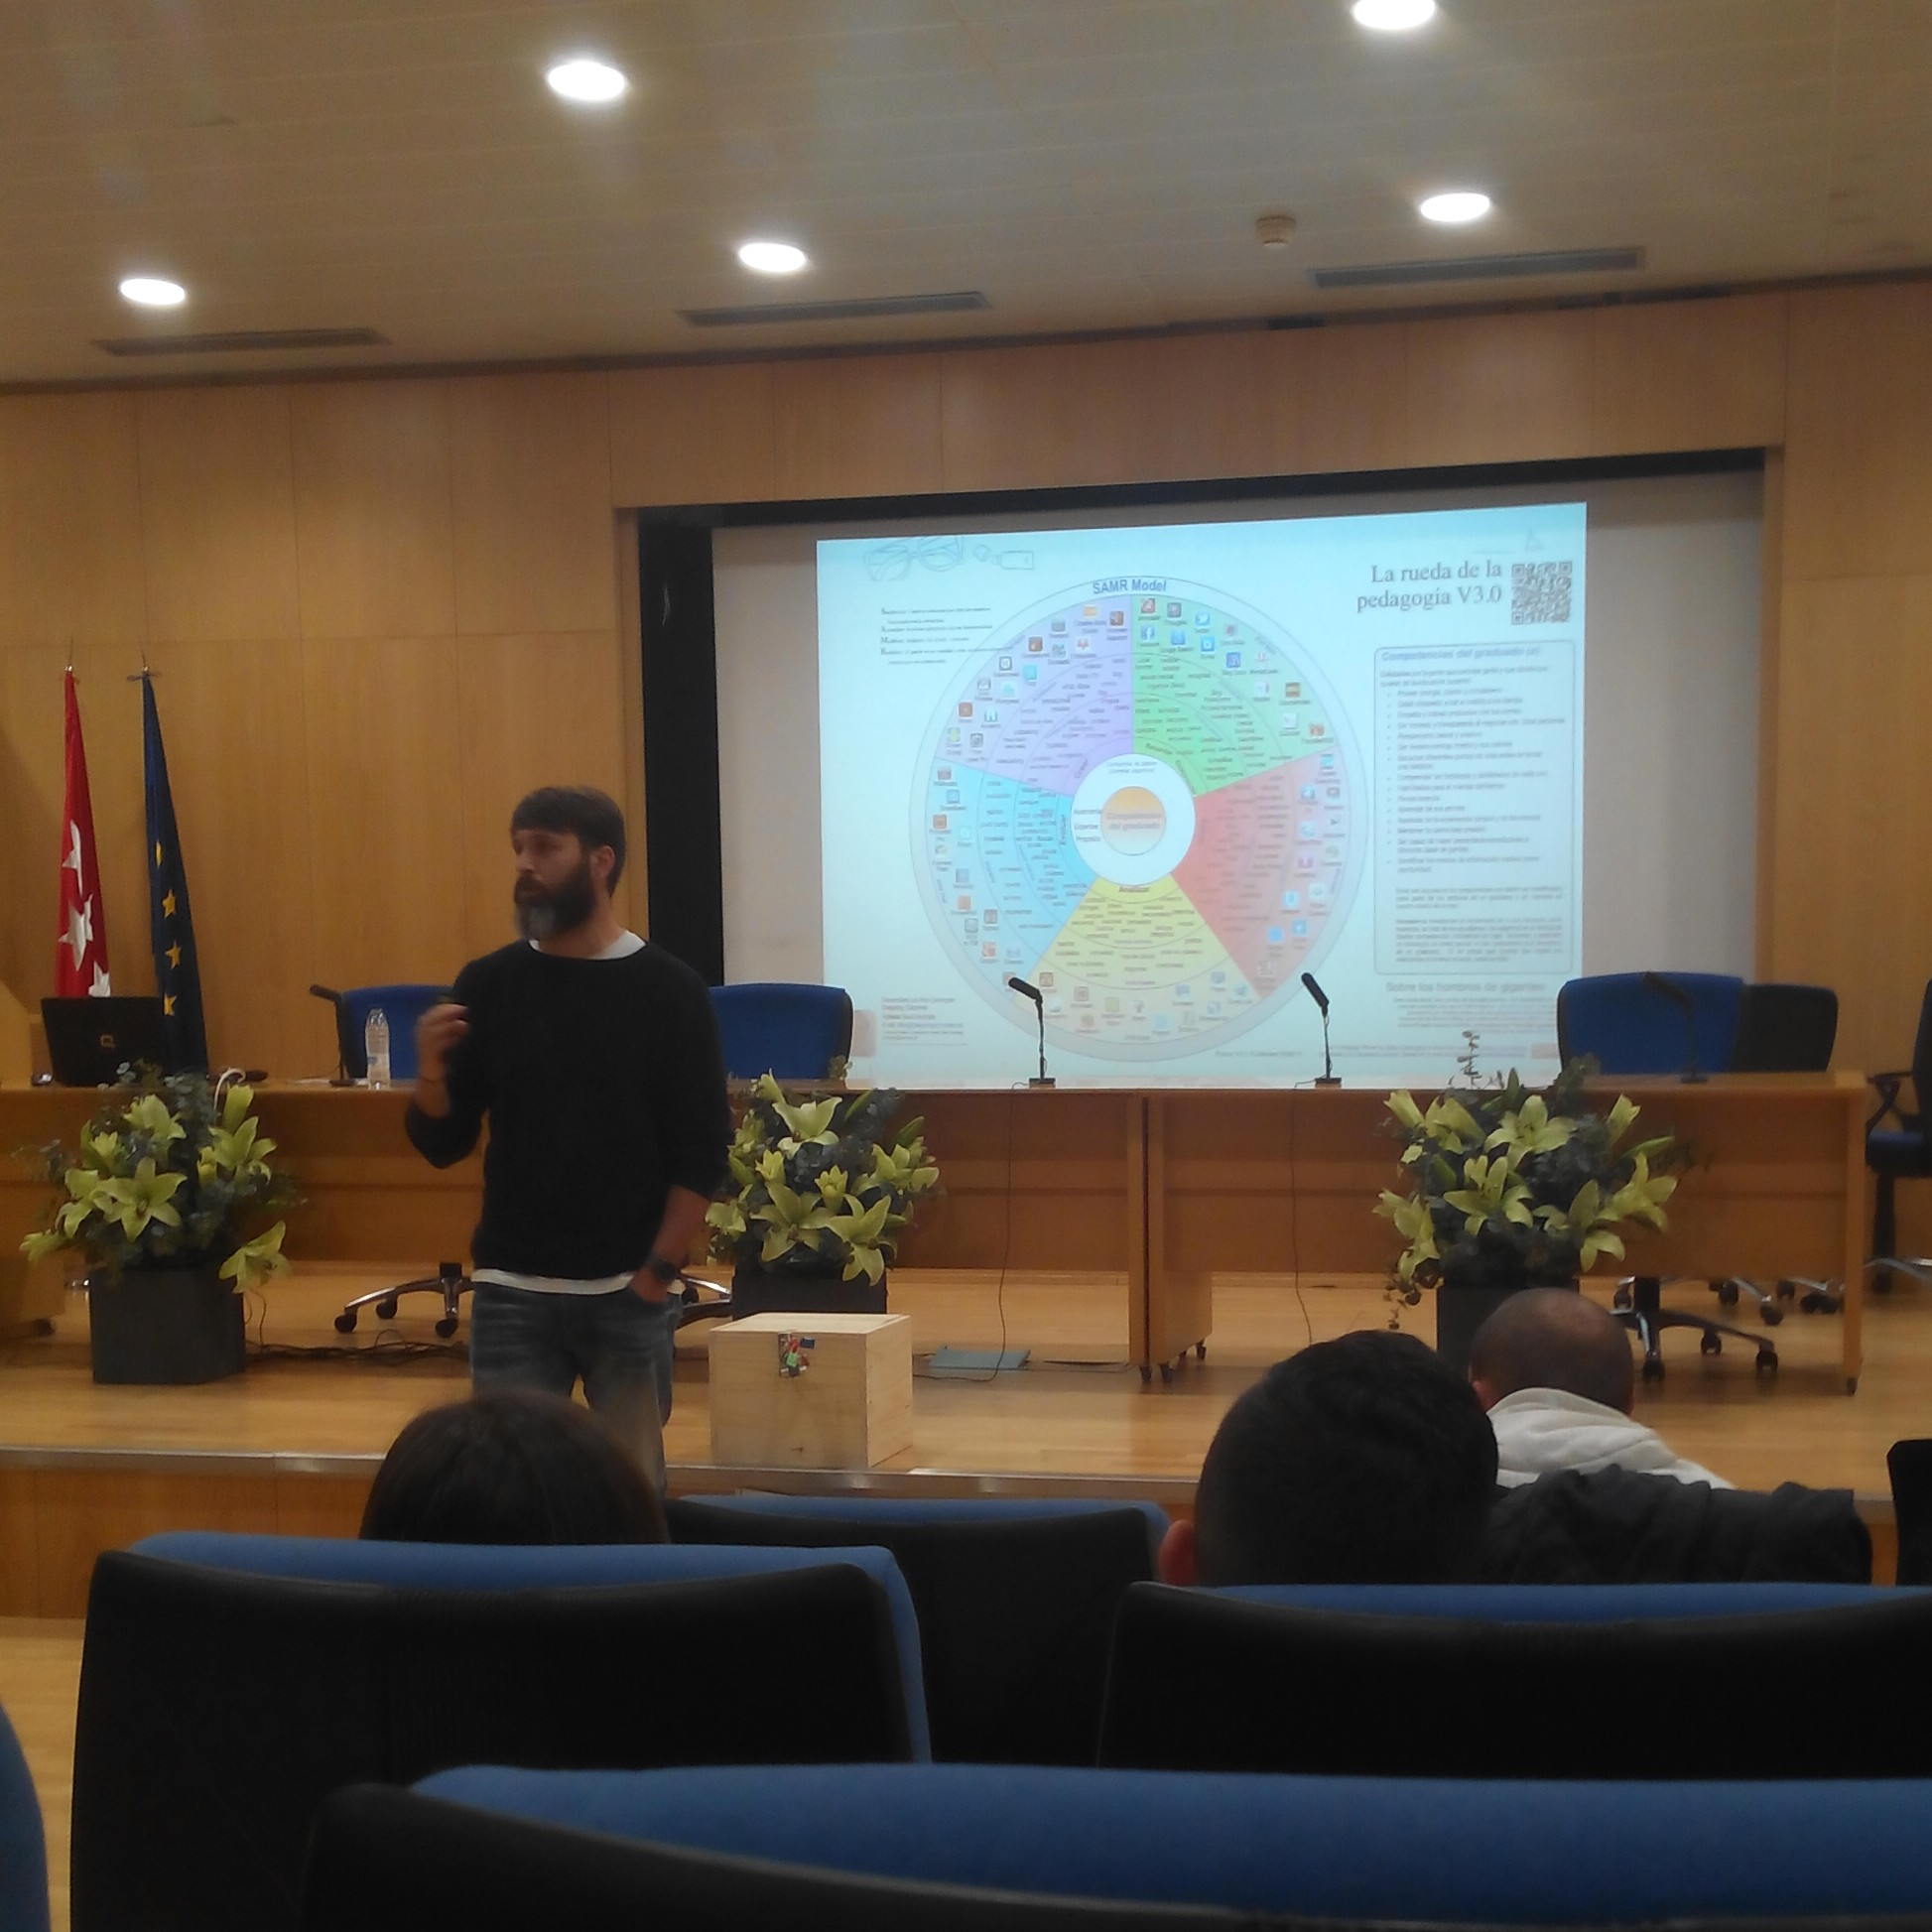
\includegraphics[scale=0.12]{img/pedron.jpg}
\caption{Comienzo de la ponencia.}
\vspace{2.0cm}
\end{leftbar}
\vspace{-2.0cm}
\end{figure}
\begin{leftbar}{\pedrocolor}

\textbf{Jonathan Bergmann y Aaron Sams}, dos profesores de química, acuñaron el término de “Flipped Classroom”. En un principio estaba orientado para aquellos alumnos que frecuentemente faltaban a clase por algún motivo personal. Con el tiempo se dieron cuenta que este mismo modelo permitía que el profesor centrara la atención en las necesidades individuales de aprendizaje de cada estudiante.

Para poder entender en qué consiste esta metodología activa de “Flipped Classroom”, Chema nos hizo llegar la siguiente definición de Raúl Santiago:

Modelo pedagógico que transfiere el trabajo de determinados procesos de aprendizaje  fuera del aula y utiliza el tiempo de clase, junto con la experiencia del docente, para facilitar y potenciar otros procesos de adquisición y práctica de conocimientos dentro del aula. 

En pocas palabras: “Lleva tu clase a cada estudiante, en cualquier momento y en cualquier lugar”

Pero la pregunta que surgió era, ¿Cómo se controla si tus alumnos hacen su trabajo fuera del aula? Chema habló que era fundamental explicar a los alumnos en qué consistía eso de la clase invertida y lo importante que es seguir unos patrones  para alcanzar el éxito que se traduce en “aprendizaje”. Según sus palabras, ellos tienen que saber que son los protagonistas de su propia película. Todos pensamos que estas palabras sobre el papel suenan bien, pero la verdad resultante en el aula es bien distinta, la prioridad de los alumnos no es aprender. Ante esto, nos presento algunas herramientas como \textbf{Playposit y EDpuzzle}:

\begin{itemize}

\item  \textbf{Playposit} El profesor puede incluir preguntas dentro de un vídeo (de origen propio o de YouTube). Lo novedoso es que el estudiante tiene que contestar primero las preguntas antes de poder continuar y sin poder avanzar a partes que todavía no ha visionado (si puede rebobinar y luego avanzar). Por otra parte el profesor puede ver en su tablero que estudiantes han realizado la tarea y los resultados. Material muy útil para utilizar en clase invertida. 

\item  \textbf{EDpuzzle} Permite convertir cualquier video en tu propia lección educativa de una forma rápida y fácil. De este modo podremos cortar un video si nos interesa solo una parte, grabar nuestra propia voz encima del video.  El resultado serán videos muy interesantes y entretenidos. 
\end{itemize}

Personalmente creo que son dos herramientas muy bien pensadas para educadores. Playposit me permite poder evaluar a mis alumnos de manera individual, identificando sus puntos débiles sobre un determinado temario.

 
A continuación, Chema nos habló de los 10  errores más comunes a la hora de crear una Flipped Classroom:

\begin{itemize}

\item Videos demasiado largos ( Un minuto por año que tenga el alumno aproximadamente) 

\item Añadir más que remplazar. Los videos deben remplazar el contenido del texto, no añadir más. 

\item Dar clase cuando los alumnos no atienden. Al principio será necesario ver los vídeos en el aula, ya que normalmente les costará cambiar de rutina. 

\item Elaborar contenido de difícil acceso. Utilizar solo un soporte para elegir los videos y materiales. Explicar donde está todo alojado y cuál es su funcionamiento. Hacerlo fácil. 

\item Inactividad de los profesores en el aula. El profesor no deberá estar cómodamente sentado durante la clase. Deberá resolver dudas de los alumnos. 

\item Rendirse. Si el método no funciona, cambia de método. 

\item No tener en cuenta los alumnos con dificultades. 

\item No hacer clases interactivas. 

\item Utilizar videos de otras personas. Hay que personalizar los videos para tus alumnos. 

\item No hacer las clases divertidas y amenas. 
\end{itemize}
Me he querido centrar en esta metodología porque opino que permite al alumno marcar su ritmo de aprendizaje. Nos alejamos de los patrones que marca el sistema educativo actual, que hace que unos alumnos vayan con la lengua fuera, mientras que otros se aburren en clase. Aquí cada alumno elige su momento de estudio.




\end{opin}

\begin{opin}{\virgicolor}{Virginia}

\subsubsection{Divulgación de las matemáticas como docentes}

En este tema vimos la importancia de la correcta divulgación de las matemáticas.  Recalco lo de correcta porque de nada sirve divulgar matemáticas si está no se hace bien y por desgracia en los medios de comunicación se cometen errores bastante importantes. Teniendo en cuenta que los principales medios de divulgación son tales medios de comunicación como, televisión, periódicos, radio e Internet creo que es de vital importancia evitarlos: ¿cómo podemos pretender que los niños se expresen bien o les exijamos unos conocimientos básicos en matemáticas si los propios periodistas cometen fallos tremendos? Uno de los ejemplos que puso Raquel y que me dejo boquiabierta fue el de Marilo con el índice de masa corporal, ya no por el hecho de que no sea capaz de usar una calculadora aun cuando le estaban explicando paso a paso como hacerlo, sino de la propia imagen que da de desinterés y despreocupación como si no pasara nada el ser incapaz de hacer algo tan sencillo como una potencia y una división.

En mi opinión, el problema con las matemáticas empieza desde pequeños en el colegio donde comienzan a percibir la asignatura como algo difícil y aburrido. Para ello la labor del profesor es de vital importancia desde las primeras etapas del aprendizaje, de forma que tiene que ser capaz de establecer una conexión entre las emociones de los alumnos y la utilidad de las matemáticas en la vida real. A día de hoy con los avances de la tecnología creo que es más sencillo ya que existen multitud de juegos matemáticos o mentales que se usan en tablets y spmartphones y que los niños estarían encantados de utilizar.

A parte de la labor del profesor, como he comentado antes, los medios de comunicación son la principal fuente de información por lo que la divulgación por parte de los mismos es imprescindible para que llegue a las distintas edades. Es cierto que existen cada vez más programas relacionados con la ciencia y las matemáticas como el Hormiguero, Orbita Laika y Desafía tu Mente. Si bien el hormiguero es un programa de éxito porque lleva famosos de distintos campos y tiene diferentes secciones el programa, los otros dos programas me temo que su audiencia dista mucho de lo que tendría que ser y más sin los comparamos con programas basura como Gran Hermano o Mujeres Hombres y viceversa.  Es una pena que la gente se una más para ver programas basura que un programa de divulgación. Siempre escucho que si lo ponen es porque la gente ve esos programas, pero también pienso que, si desaparecieran todos esos programas basura y se pusieran más programas de entretenimiento relacionados con la ciencia y su divulgación y en un horario más apto para niños, seguro que se crearían unas inquietudes diferentes a esos niños, tendrían más ganas de aprender cosas curiosas e interesantes que buscar la forma de ganar más dinero trabajando menos.

Dentro de los libros, videos y/o artículos de divulgación matemática que vimos en clase quiero destacar los siguientes:

\begin{itemize}

\item La sección de Raúl Ibánez sobre matemáticas en Orbita Laika ya que Raúl consigue ganar el premio más importante de divulgación científica en España. Además es el creador y director de una página muy interesante, Divulgamat: \url{http://www.divulgamat.net/} 

\item Universo matemático que fue galardonada en el Festival Internacional Científico de Pekín con el Premio a la divulgación científica. 

\item El libro de Mateschef ya que el libro trata de hacer relaciones curiosas entre geometría y cocina, y las matemáticas y la cocina son dos cosas que me encantan así, que mejor forma que unir las dos. En el campo de la cocina y teniendo en cuenta el nombre de este libro, recuerdo siempre como en el programa de MasterChef cuando hacen postres recalcan siempre que “la repostería es matemática pura”. 

\item Matemáticas invisibles: muy interesante el artículo de las plantas carnívoras: \url{http://www.agenciasinc.es/Noticias/Las-plantas-carnivoras-utilizan-las-matematicas-para-cazar-a-sus-presas} 

\item El mundo con mirada matemática: a parte de lo que vimos en clase me gustaría añadir una web en la que se incluyen edificios famosos inspirados en las matemáticas: \url{http://www.metrocuadrado.com/noticias/especiales/edificios-famosos-inspirados-en-las-matematicas-664} 
\end{itemize}


Además de todos los libros que vimos en clase de los distintos divulgadores y todos los programas de los que hablamos, me gustaría aportar otros programas que yo he visto y que me parece muy interesantes como son: Mythbusters (Cazadores de mitos), por el Discovery Channel, y Brain Games (Juegos mentales) por National Geographic. El primero, está más relacionado con la divulgación científica y consistía en comprobar la veracidad de las leyendas urbanas y otras creencias usando para ello métodos científicos. El segundo, en realidad podría haberlo incluido cuando se trató la neurodidáctica ya que en este programa se explora los componentes del cerebro humano y su funcionamiento empleando expertos en ciencia cognitiva, neurociencia y psicología. No obstante, son dos programas muy interesantes a la vez que entretenidos, por lo que habría que promocionar más este tipo de programas.

A parte de todos los divulgadores que comentó Raquel quiero hablar de Eduardo Sáenz de Cabezón, un matemático que intenta relacionar las matemáticas con la magia y el humor. Además, es uno de los participantes de un grupo de matemáticos, biológos, científicos... que hacen monólogos. Aquí muestro el link de dos noticias sobre él y las matemáticas:

\url{http://www.abc.es/sociedad/abci-eduardo-sanchez-cabezon-matematico-desvela-magia-numeros-201512180154_noticia.html}

En este artículo Eduardo reflexiona acerca de la tendencia de la gente a renegar de las matemáticas: “Quizá solo falta perderles el miedo, acercarse de forma diferente a la que estamos acostumbrados”.

\url{http://www.nacion.com/vivir/ciencia/hombre-saca-chistes-matematica_0_1565443465.html}

En el vídeo que sale en este artículo me parece divertido su consejo para hacer un regalo a alguien que le quieres demostrar que tu amor es para siempre: “Si quieres decir a alguien que le quieres para siempre, regálale un teorema en lugar de un diamante”. Para finalizar recalca que hay que cambiar la educación matemática actual.

Y por último la página del grupo de monologuistas al que pertenece y de las actividades que realizan que me parece una labor muy importante, interesante y divertida para dar a conocer los diferentes entresijos de la ciencia:

\url{http://www.bigvanscience.com/tbvt.html}

En definitiva, hay multitud de formas de disfrutar de la ciencia en general y las matemáticas en particular, y para hacer uso de dichas formas, el deber de padres, profesores y medios de comunicación es conseguir inquietar y emocionar las mentes de los niños, para lo que antes son los propios adultos los que tendrían que conseguir emocionarse.

\end{opin}
